\chapter{Background}
\label{ch:background}

\section{Reinforcement learning}
Given uncertian and possibly varying parameters an agent choses
its actions based on prior knowledge and by repeated trials. The very first action
will be chosen by random and the agent will then recieve a reward or
penalty from the environment. This feedback will then be used to update the expected reward
from that perticular action. By repeatedly chosing the actions and receiving feedback
from the environment, as pictured in figure~\ref{fig:rlearn}, the agent is able to
decide which action is the most profitable. 

If the environment does in fact have varying parameters, meaning that the reward
is normally distributed, the agent have to weigh exploration against
explotation. Given two choices, if the agent choses option A and then option B one time each and
option A gives a higher reward it does not necessarily mean that option A gives the highest
reward over time. Thus the agent have to decide on wether to continue
to test both options, to get a clearer picture of which option is the better one, or to repeatedly
select the option it believes is the best one to maximize profit. 

\begin{figure}[ht]
    \centering
    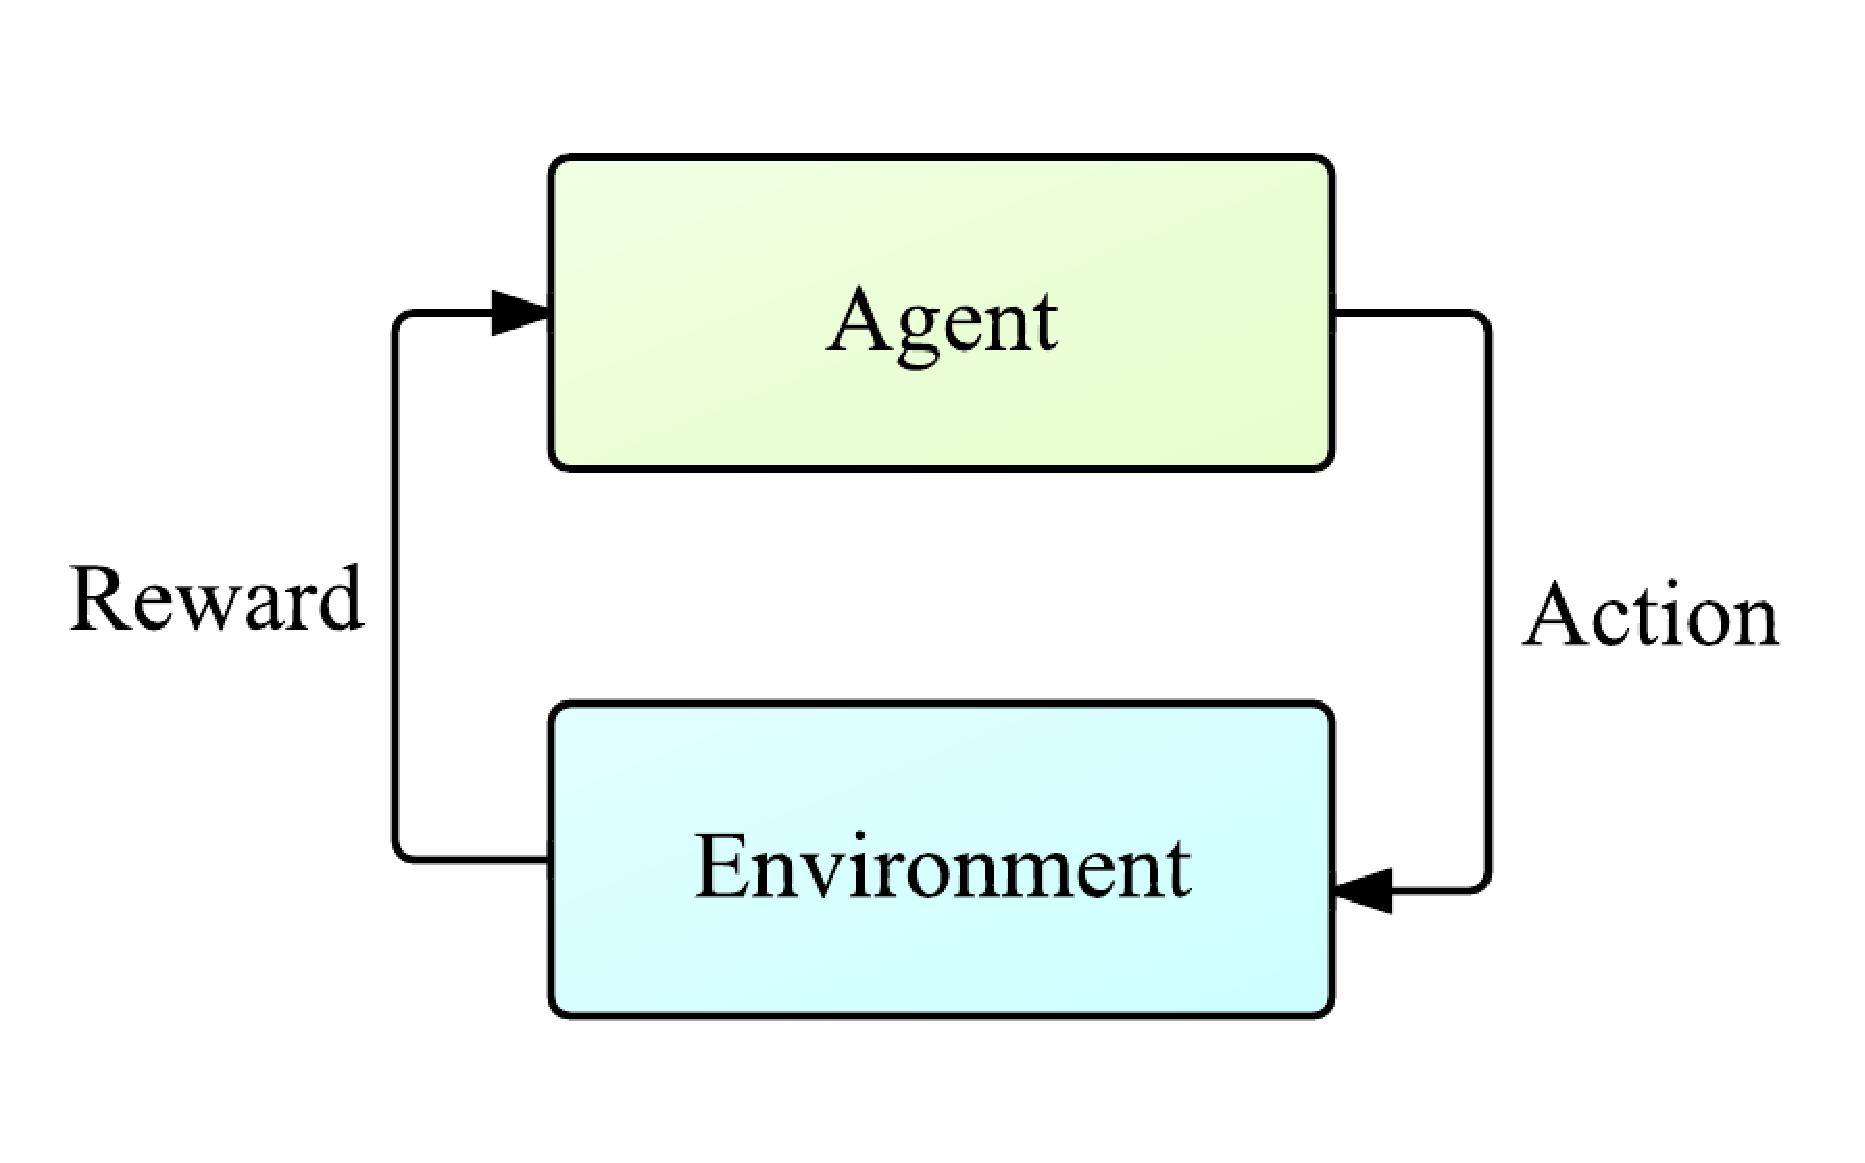
\includegraphics[width=8cm]{images/ReinforcementLearning}
    \label{fig:rlearn}
    \caption{Reinforcement learning}
\end{figure}

\section{The multi-armed bandit problem}
\textbf{Define regret (total and instant)}
A popular and surprisingly fitting way to model stochastic optimization problems 
is through the multi-armed bandit scenario. Imagine, if you will, the iconic 
gambling machine to be found in any casino. Only this apparatus has not one, but 
many arms with which a player may try her luck. Oh, but which arm to choose? 
With so many possible choices, a strategy for optimising the machine’s payout 
must be employed. 

Before any arm-pulling has been done, nothing is known about the possible 
payoffs from the multitude of available arms exept that some arms are better 
than others -- obviously our player will profit the most from playing only the 
best arm. And so, it comes to this: she must make a tradeoff between exploration 
-- discovering which arm is truly the best one -- and exploitation -- actually 
picking the best arm.

More specifically, in this paper we look at Gaussian bandits.
This means that arms are normally distributed, and each arm is described by a mean and standard deviation.
Furthermore, seeing as the normal distribution is self-conjugate, this allows for the
use of normal distributions to describe the arm estimates used in the LTS algorithm.

\section{The Goore Game}
Introduced by Tsetlin in 1973, the Goore game is a cooperation game where each  
player is not privy to information on the other players choices. It can be 
described as a voting process where the referee knows the correct answer, and 
the players cast their votes as simple ‘yes’ or ‘no’. The correct answer is a 
certain number of yes’s and no’s, and players are rewarded based on how close 
they collectively are to the ideal solution.

\begin{figure}[h]
\centering
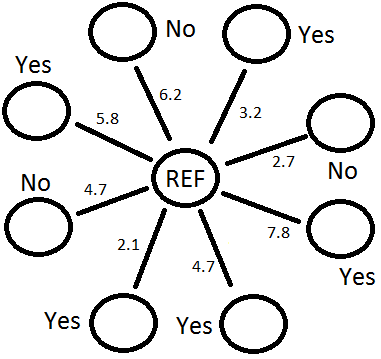
\includegraphics[height=70mm,width=70mm]{images/goore_game.png}
\caption{Eight Player Goore Game}
\label{fig:gg}
\end{figure}
At the start of the game all participants selects an action at random, as seen in figure \ref{fig:gg}. The referee
gathers all the votes and based on a unimodal performance criterion it decides on
the amount of reward each player will receive. The players will then use the reward they received from the
referee to decide on wether to chose another action or to stick to their previous one. As seen in figure \ref{fig:gg},
some players receive a higher reward than other while chosing the same action and this is a part
of the uncertainty in the Goore Game, that a player can make the correct choice and stil receive a low
reward.

Another factor that makes the game more difficult is that only the referee knows off the unimodal performance criterion.
The players simply votes and receives a reward as feedback. As the name 'unimodal' suggest there is only a single
amount of 'yes' and 'no' that yeilds the highest likely award. An example of such a function can be seen in figure \ref{fig:gfunc}.
In the figure $\lambda$ is the amount of players that vote yes and $\lambda^*$ is the target value which is when the referee
likely will provide the highest rewards. Thus, if the players reach the target value they are not ensured a high reward, however
the players are most likely to receive a high reward by staying at this configuration.
\begin{figure}[h]
\centering
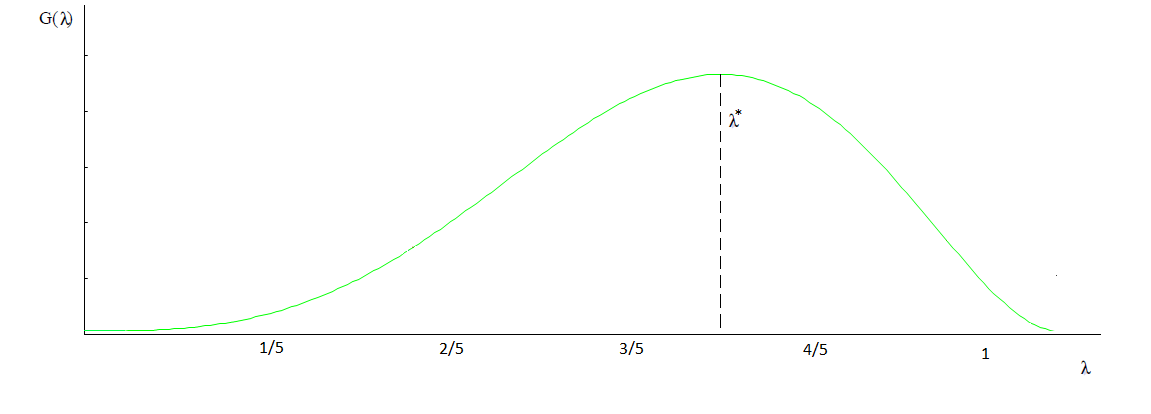
\includegraphics[height=50mm,width=150mm]{images/gfunc.png}
\caption{An unimodal performance criterion}
\label{fig:gfunc}
\end{figure}
A final factor that increases the difficulty of the game is that a players choice is affected by the other
players choices. Lets say that ten players all select 'no' at the first round and that the performance 
criterion is as shown in figure \ref{fig:gfunc}. The probability of
each individual player receiving a high reward would be fairly low and thus most of them
are likely to chose another action. Nevertheless, some players  could received a decent reward
and chosen to stick to their previous action. Even if the players
chose the ideal solution during the first round it is likely that not all players would
receive a reward and thus it takes some time to explore all options before the players
converge on the ideal solution, which in this case would be seven 'yes' and three 'no' as seen in the figure.

\section{Local Thompson sampling}
Local Thompson sampling \cite{May2011} is based on a sampling technique pioneered by Thompson \cite{Thompson1933} in 1933. 
The method is Bayesian in nature, in that it uses new information to update probability estimates, but avoids the computational intractability that is often the drawback of Bayesian methods.
For every available arm it keeps a distribution estimate, which is 
updated based on received reward. The use of Thompson sampling in the bandit 
setting depends on a parameter known as observation noise, $\sigma_{ob}$, which 
is assigned a value based on how much new information is to be trusted. A low 
observation noise signifies that new information should be considered 
trustworthy, while a high value means that observations are insecure.

After receiving a reward $r_i$ by pulling arm $i$ the bandit is updated. The mean and variance
is calculated as follows \cite{Murphy2007}:
\begin{displaymath}
\mu_i [t + 1] = \frac{\sigma_i^2 [t] \cdot r_i + \sigma_{ob}^2 \cdot \mu_i [t]}{\sigma_i^2 [t] + \sigma_{ob}^2}
\end{displaymath}

\begin{displaymath}
\sigma_i^2 [t + 1] = \frac{\sigma_i^2 [t] \sigma_{ob}^2}{\sigma_i^2 [t] + \sigma_{ob}^2}
\end{displaymath}
Where $\sigma_i^2 [t + 1]$ and $\mu_i [t + 1]$ is the variance and mean of the updated arm and
$\sigma_i^2 [t]$ and $\mu_i [t]$ is the variance and mean of the arm in its previous state.

\begin{figure}[htbp]
    \centering
% Haskell code to generate data:
% let var v ob = let vv = (v*ob)/(v+ob) in vv : var vv ob
% let ppB b = unlines $ map ppL b
% let ppL (t,a,b,c) = show t ++ " " ++ show a ++ " " ++ show b ++ " " ++ show c
% writeFile "est.txt" . unlines . map ppB . transpose 
%   $ map (\(est, ob) -> (zip4 (var est ob) ([1..10000]) (repeat est) (repeat ob)))
%         [(est, ob) | est <- [2500],
%                      ob <- ([0.001,0.002, 0.003, 0.006, 0.01, 0.03,0.06] ++ [0.1,0.2..3.0])]

%    Let's not recompile this thing all the time.
%    \begin{gnuplot}[terminal=epslatex,terminaloptions=color solid]
%    set grid
%    set ylabel "[r]{\\shortstack{Observation noise \\\\ ($\\sigma_{ob}^2$)}}" offset 6,-2
%    set xlabel 'Rounds' offset 0,-0.5
%    set zlabel 'Variance estimate ($\hat{\sigma}^2$)' rotate offset -0.5,0
%    set xyplane 0
%    set log z; set log cb
%    set xrange [0:1000]
%    set zrange [1e-06:3]
%    set ytics 0.4 offset 0,-0.5
%    set xtics offset 0,-0.5
%     set palette model CMY rgbformulae 7,5,15
%    splot 'est.txt' using 2:(column(4) < 1.5 ? column(4) : 1/0):(column(3) == 2500.0 ? column(1) : 1/0) every :::::1000 with pm3d title "" \
%    ,'est.txt' using 2:(column(4)<1.5?column(4):1/0):(column(3)==2500.0?column(1):1/0) every 2:100::50::1001 with line lt -1 lw 1 title "" \
%    ,'est.txt'       using 2:(column(4) < 1.5 ? column(4) : 1/0):(column(3) == 2500.0 ? column(1) : 1/0) every 2:10::::70  with line lt -1 lw 1 title ""
%    \end{gnuplot}
%    % GNUPLOT: LaTeX picture with Postscript
\begingroup
  \makeatletter
  \providecommand\color[2][]{%
    \GenericError{(gnuplot) \space\space\space\@spaces}{%
      Package color not loaded in conjunction with
      terminal option `colourtext'%
    }{See the gnuplot documentation for explanation.%
    }{Either use 'blacktext' in gnuplot or load the package
      color.sty in LaTeX.}%
    \renewcommand\color[2][]{}%
  }%
  \providecommand\includegraphics[2][]{%
    \GenericError{(gnuplot) \space\space\space\@spaces}{%
      Package graphicx or graphics not loaded%
    }{See the gnuplot documentation for explanation.%
    }{The gnuplot epslatex terminal needs graphicx.sty or graphics.sty.}%
    \renewcommand\includegraphics[2][]{}%
  }%
  \providecommand\rotatebox[2]{#2}%
  \@ifundefined{ifGPcolor}{%
    \newif\ifGPcolor
    \GPcolortrue
  }{}%
  \@ifundefined{ifGPblacktext}{%
    \newif\ifGPblacktext
    \GPblacktexttrue
  }{}%
  % define a \g@addto@macro without @ in the name:
  \let\gplgaddtomacro\g@addto@macro
  % define empty templates for all commands taking text:
  \gdef\gplbacktext{}%
  \gdef\gplfronttext{}%
  \makeatother
  \ifGPblacktext
    % no textcolor at all
    \def\colorrgb#1{}%
    \def\colorgray#1{}%
  \else
    % gray or color?
    \ifGPcolor
      \def\colorrgb#1{\color[rgb]{#1}}%
      \def\colorgray#1{\color[gray]{#1}}%
      \expandafter\def\csname LTw\endcsname{\color{white}}%
      \expandafter\def\csname LTb\endcsname{\color{black}}%
      \expandafter\def\csname LTa\endcsname{\color{black}}%
      \expandafter\def\csname LT0\endcsname{\color[rgb]{1,0,0}}%
      \expandafter\def\csname LT1\endcsname{\color[rgb]{0,1,0}}%
      \expandafter\def\csname LT2\endcsname{\color[rgb]{0,0,1}}%
      \expandafter\def\csname LT3\endcsname{\color[rgb]{1,0,1}}%
      \expandafter\def\csname LT4\endcsname{\color[rgb]{0,1,1}}%
      \expandafter\def\csname LT5\endcsname{\color[rgb]{1,1,0}}%
      \expandafter\def\csname LT6\endcsname{\color[rgb]{0,0,0}}%
      \expandafter\def\csname LT7\endcsname{\color[rgb]{1,0.3,0}}%
      \expandafter\def\csname LT8\endcsname{\color[rgb]{0.5,0.5,0.5}}%
    \else
      % gray
      \def\colorrgb#1{\color{black}}%
      \def\colorgray#1{\color[gray]{#1}}%
      \expandafter\def\csname LTw\endcsname{\color{white}}%
      \expandafter\def\csname LTb\endcsname{\color{black}}%
      \expandafter\def\csname LTa\endcsname{\color{black}}%
      \expandafter\def\csname LT0\endcsname{\color{black}}%
      \expandafter\def\csname LT1\endcsname{\color{black}}%
      \expandafter\def\csname LT2\endcsname{\color{black}}%
      \expandafter\def\csname LT3\endcsname{\color{black}}%
      \expandafter\def\csname LT4\endcsname{\color{black}}%
      \expandafter\def\csname LT5\endcsname{\color{black}}%
      \expandafter\def\csname LT6\endcsname{\color{black}}%
      \expandafter\def\csname LT7\endcsname{\color{black}}%
      \expandafter\def\csname LT8\endcsname{\color{black}}%
    \fi
  \fi
  \setlength{\unitlength}{0.0500bp}%
  \begin{picture}(7200.00,5040.00)%
    \gplgaddtomacro\gplbacktext{%
      \csname LTb\endcsname%
      \put(942,1180){\makebox(0,0){\strut{} 0}}%
      \csname LTb\endcsname%
      \put(1590,1061){\makebox(0,0){\strut{} 200}}%
      \csname LTb\endcsname%
      \put(2238,942){\makebox(0,0){\strut{} 400}}%
      \csname LTb\endcsname%
      \put(2886,824){\makebox(0,0){\strut{} 600}}%
      \csname LTb\endcsname%
      \put(3533,705){\makebox(0,0){\strut{} 800}}%
      \csname LTb\endcsname%
      \put(4180,586){\makebox(0,0){\strut{} 1000}}%
      \csname LTb\endcsname%
      \put(4398,646){\makebox(0,0){\strut{} 0}}%
      \csname LTb\endcsname%
      \put(4866,904){\makebox(0,0){\strut{} 0.4}}%
      \csname LTb\endcsname%
      \put(5333,1161){\makebox(0,0){\strut{} 0.8}}%
      \csname LTb\endcsname%
      \put(5801,1418){\makebox(0,0){\strut{} 1.2}}%
      \csname LTb\endcsname%
      \put(6268,1675){\makebox(0,0){\strut{} 1.6}}%
      \put(920,1384){\makebox(0,0)[r]{\strut{} 1e-06}}%
      \put(920,1702){\makebox(0,0)[r]{\strut{} 1e-05}}%
      \put(920,2020){\makebox(0,0)[r]{\strut{} 0.0001}}%
      \put(920,2337){\makebox(0,0)[r]{\strut{} 0.001}}%
      \put(920,2654){\makebox(0,0)[r]{\strut{} 0.01}}%
      \put(920,2972){\makebox(0,0)[r]{\strut{} 0.1}}%
      \put(920,3289){\makebox(0,0)[r]{\strut{} 1}}%
      \put(171,2562){\rotatebox{-270}{\makebox(0,0){\strut{}Variance estimate ($\hat{\sigma}^2$)}}}%
    }%
    \gplgaddtomacro\gplfronttext{%
      \csname LTb\endcsname%
      \put(2198,721){\makebox(0,0){\strut{}Rounds}}%
      \put(6821,717){\makebox(0,0)[r]{\shortstack{Observation noise \\ ($\sigma_{ob}^2$)}}}%
      \put(171,2562){\rotatebox{-270}{\makebox(0,0){\strut{}Variance estimate ($\hat{\sigma}^2$)}}}%
      \put(6641,2280){\makebox(0,0)[l]{\strut{} 1e-06}}%
      \put(6641,2498){\makebox(0,0)[l]{\strut{} 1e-05}}%
      \put(6641,2717){\makebox(0,0)[l]{\strut{} 0.0001}}%
      \put(6641,2935){\makebox(0,0)[l]{\strut{} 0.001}}%
      \put(6641,3154){\makebox(0,0)[l]{\strut{} 0.01}}%
      \put(6641,3372){\makebox(0,0)[l]{\strut{} 0.1}}%
      \put(6641,3591){\makebox(0,0)[l]{\strut{} 1}}%
      \put(6641,3810){\makebox(0,0)[l]{\strut{} 10}}%
    }%
    \gplbacktext
    \put(0,0){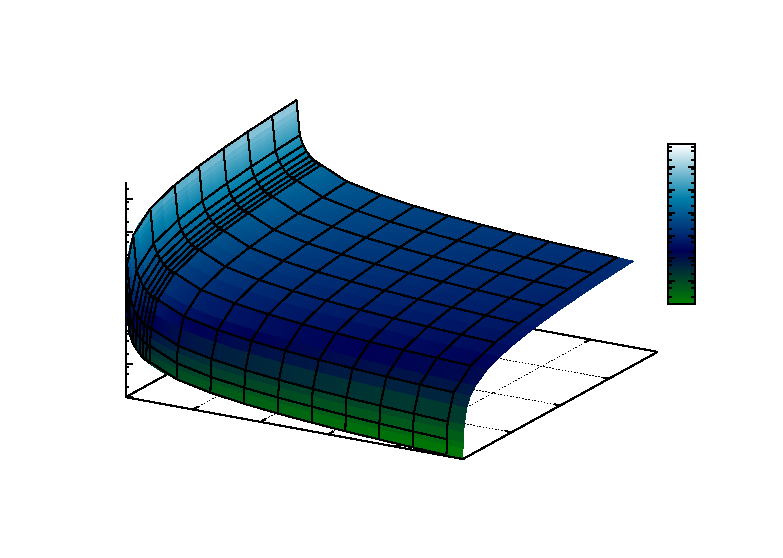
\includegraphics{ob-var-fig1}}%
    \gplfronttext
  \end{picture}%
\endgroup

\begin{gnuplot}[terminal=epslatex,terminaloptions=color solid]
    set style data lines
    set log y
    set xlabel "Rounds"
    set ylabel '$\hat{\sigma}^2$'
    set xtics 1,100,1000
    plot [1:1000] [*:1] for [o in "1.0 1.0e-3"] 'est.txt' using ($4==o?$2:NaN):1 title 'OB = '.o
    \end{gnuplot}
\caption{Variance as a function of time}
\label{fig:variance}
\end{figure}


\begin{figure}[htbp]
    \hspace*{-2.5cm}
    \begin{minipage}[c]{0.39\textwidth}
    \begin{gnuplot}[terminal=epslatex,terminaloptions=color solid]
    set style data lines
    set grid
    set xlabel "Observation noise"
    set ylabel "Total regret"
    set xrange [0.15:0.95]
    plot "../data/bruteforce/good-5.0,2.0\_bad-4.0,4.0\_est-10.0,0.5\_num-2\_obstart-0.15\_obend-0.95\_obstep-0.01\_rounds-10000\_reps-10000.data" using 2:(column(1)==1000?(5000-column(3)):(1/0)) title ""
    \end{gnuplot}
    \end{minipage}
    \hspace*{7.5cm}
    \begin{minipage}[c]{0.49\textwidth}
    \banditsetup{5.0}{2.0}{4.0}{4.0}{2}{1000}
    \end{minipage}
\caption{Resulting total regret from varying observation noise.}
\label{fig:regretob}
\end{figure}

Figure~\ref{fig:regretob} illustrates why, when using LTS, it is important to make a good choice of observation noise.
In this case we see that the total regret achieved increases rapidly when the value is set too low, while it increases slightly as we move past the optimum.
With different setups we see similar results, although the slope after the optimum may be steeper or closer to zero.


\section{UCB1-Tuned}
In addition to local Thompson sampling, we implemented the UCB1 algorithm for 
comparing optimised Thompson samplers.

UCB1 \cite{Auer02UCB1} (Upper Confidence Bound) is a well-known algorithm for multi-armed bandits.
It is popular due to being very simple and reasonably performant. In comparison 
to LTS, it does not require any constant parameters, and in place of a given 
start estimate for the available arms the fist $K$ rounds are dedicated to 
initialising the arm estimates by playing every arm once.

UCB1-Tuned is a version of UCB1 that takes into consideration the estimate variance in addition to the estimate mean.
This should cause it to work better in practice.
In the remainder of this report, UCB1 means this improved algorithm.

The UCB1-Tuned strategy is simply to play the arm with index $i$ such that
\begin{displaymath}
    i = \operatorname*{argmax}_{j \in \{ 1..K \}} \left(\hat{\mu}_j + 
    \sqrt{\frac{\ln{n}}{n_j} \min(\frac{1}{4},\hat{V}_j)}\right)
\end{displaymath}
where 
\begin{displaymath}
    \hat{V}_j = \hat{\sigma}_j^2 + \sqrt{\frac{2\ln{n}}{n_j}}\text{.}
\end{displaymath}

$K$ is the number of available arms, $n_j$ the numer of times arm $j$ has 
been played, $n$ is the total number of plays, and $\hat{\mu}_j 
=\frac{(\text{cumulative reward for arm j})}{n_j}$.

% \section{Sample stuff}
% Some simple and useful latex formatting.
% 
% \subsection{Quotations and citing}
% It is explained in detail in \cite[Ch.20]{Norvig03} that
% 
% \begin{quotation}
% \noindent \textit{``the true hypothesis eventually dominates the Bayesian 
% predication. For any fixed prior that does not rule out the true hypothesis, the 
% posterior probability of any false hypothesis will eventually vanish, simply 
% because the probability of generating ``uncharacteristic'' data indefinitely is 
% vanishingly small.''}
% \end{quotation}
% 
% \subsection{Figures}
% This distribution, and its probability density function, is displayed in Figure 
% \ref{fig:gaussian_distr_pdf}.
% \begin{figure}[ht]
%     \center\includegraphics[width=10cm]{images/normal_distr_pdf}	
%     \label{fig:gaussian_distr_pdf}
%     \caption{The Normal distribution PDF.}
% \end{figure}
% 
% \subsection{Equations}
% By using these probabilities, and Bayes formula, we can derive the Bayes 
% classifier.
% \begin{equation}
%     P(\omega_i | \boldsymbol{x}, \mathcal{X}) = \frac{p(\boldsymbol{x}|\omega_i, 
%     \mathcal(X))P(\omega_i|\mathcal{X})}{\sum_{j=1}^{c}p(\boldsymbol{x}|\omega_j, 
%     \mathcal{X})P(\omega_j|\mathcal{X})},
%     \label{eq:bayes_formula_1}
% \end{equation}
% 
% when we can separate the training samples by class into $c$ subsets 
% $\mathcal{X}_1, \ldots, \mathcal{X}_c$, with the samples in $\mathcal{X}_i$ 
% belonging to $\omega_i$.
% 

